\documentclass[12pt,a4paper]{article}
\usepackage[british]{babel}
\usepackage[a4paper,top=2cm,bottom=2cm,left=2.5cm,right=2.5cm,marginparwidth=1.75cm]{geometry}


\usepackage{float}
\usepackage{amsmath}
\usepackage{graphicx}
\graphicspath{ {./images/} }
\usepackage[colorlinks=true, allcolors=blue]{hyperref}
\usepackage{hyperref}
\usepackage{orcidlink}
\usepackage[title]{appendix}
\usepackage{mathrsfs}
\usepackage{amsfonts}
\usepackage{booktabs} % For \toprule, \midrule, \botrule
\usepackage{caption}  % For \caption
\usepackage{threeparttable} % For table footnotes
\usepackage{algorithm}
\usepackage{algorithmicx}
\usepackage{algpseudocode}
\usepackage{listings}
\usepackage{enumitem}
\usepackage{chngcntr}
\usepackage{booktabs}
\usepackage{lipsum}
\usepackage{subcaption}
\usepackage{authblk}
\usepackage[T1]{fontenc}    % Font encoding
\usepackage{csquotes}       % Include csquotes
\usepackage{diagbox}
\usepackage{xcolor}
\usepackage{bera}
% Customize line spacing
\usepackage{setspace}
\onehalfspacing % 1.5 line spacing

% Redefine section and subsection numbering format
\usepackage{titlesec}
\titleformat{\section} % Redefine section numbering format
  {\normalfont\Large\bfseries}{\thesection.}{1em}{}
  
% Customize line numbering format to right-align line numbers
\usepackage{lineno} % Add the lineno package

%Following 3 commands make right side line numbers

%\renewcommand\linenumberfont{\normalfont\scriptsize\sffamily\color{blue}}
%\rightlinenumbers % Right-align line numbers
%\linenumbers % Enable line numbering

% Define a new command for the fourth-level title.
\newcommand{\subsubsubsection}[1]{%
  \vspace{\baselineskip}% Add some space
  \noindent\textbf{#1\\}\quad% Adjust formatting as needed
}
% Change the position of the table caption above the table
\usepackage{float}   % for customizing caption position
\usepackage{caption} % for customizing caption format

\colorlet{punct}{red!60!black}
\definecolor{background}{HTML}{EEEEEE}
\definecolor{delim}{RGB}{20,105,176}
\colorlet{numb}{magenta!60!black}
\definecolor{codegreen}{rgb}{0,0.6,0}
\definecolor{codegray}{rgb}{0.5,0.5,0.5}
\definecolor{codepurple}{rgb}{0.58,0,0.82}
\definecolor{backcolour}{rgb}{0.95,0.95,0.92}

\lstdefinestyle{mystyle}{
    backgroundcolor=\color{backcolour},   
    commentstyle=\color{codegreen},
    keywordstyle=\color{magenta},
    numberstyle=\tiny\color{codegray},
    stringstyle=\color{codepurple},
    basicstyle=\ttfamily\footnotesize,
    breakatwhitespace=false,         
    breaklines=true,                 
    captionpos=b,                    
    keepspaces=true,                 
    numbers=left,                    
    numbersep=5pt,                  
    showspaces=false,                
    showstringspaces=false,
    showtabs=false,                  
    tabsize=2
}

\lstdefinelanguage{json}{
    basicstyle=\normalfont\ttfamily,
    numbers=left,
    numberstyle=\scriptsize,
    stepnumber=1,
    numbersep=8pt,
    showstringspaces=false,
    breaklines=true,
    frame=lines,
    backgroundcolor=\color{background},
    literate=
     *{0}{{{\color{numb}0}}}{1}
      {1}{{{\color{numb}1}}}{1}
      {2}{{{\color{numb}2}}}{1}
      {3}{{{\color{numb}3}}}{1}
      {4}{{{\color{numb}4}}}{1}
      {5}{{{\color{numb}5}}}{1}
      {6}{{{\color{numb}6}}}{1}
      {7}{{{\color{numb}7}}}{1}
      {8}{{{\color{numb}8}}}{1}
      {9}{{{\color{numb}9}}}{1}
      {:}{{{\color{punct}{:}}}}{1}
      {,}{{{\color{punct}{,}}}}{1}
      {\{}{{{\color{delim}{\{}}}}{1}
      {\}}{{{\color{delim}{\}}}}}{1}
      {[}{{{\color{delim}{[}}}}{1}
      {]}{{{\color{delim}{]}}}}{1},
}

\lstset{style=mystyle}
% Define the unnumbered list
\makeatletter
\newenvironment{unlist}{%
  \begin{list}{}{%
    \setlength{\labelwidth}{0pt}%
    \setlength{\labelsep}{0pt}%
    \setlength{\leftmargin}{2em}%
    \setlength{\itemindent}{-2em}%
    \setlength{\topsep}{\medskipamount}%
    \setlength{\itemsep}{3pt}%
  }%
}{%
  \end{list}%
}
\makeatother

% Suppress the warning about \@parboxrestore
\pdfsuppresswarningpagegroup=1


%-------------------------------------------
% Paper Head
%-------------------------------------------
\title{The network of music collaborations: Exploring how collaborations influence music genres and artist popularity}

\author[1]{Ty Irving}
\author[2]{Wasif Ud Dowlah}
\author[3]{Haoyang Shi}
\affil[1]{\small CPSC 572, 30105319}
\affil[2]{CPSC 572, 30130706}
\affil[3]{CPSC 572, 30105296}

\date{April 4th, 2024}  % Remove date

\begin{document}
\maketitle

\section{Project Summary}
  Historically and currently collaborations between artists play a pivotal role in shaping how music is created and shared to individuals.  Our project looks into the network of Spotify collaborations and aims to try and discern the impact of collaborations on artists' popularity.  The network that is intended to display the impact of collaborations is an undirected network between artists which intends on displaying the collaboration of artists when they collaborate on songs together this demonstrates the ability of collaboration on artist performance when studied.  The data in which this network is derived is gathered from the \href{https://developer.spotify.com/documentation/web-api}{Spotify Web API} which contains the artists songs and collaborations which will be gone through to create edges for the undirected network.  The resulting network demonstrated that the artists mainly collaborated with a few main artists in the community and generally the popularity of the artists who collaborated with each other were similar.  Due to the results that were gathered it was obvious that the impact of collaboration tends to be related with individuals who had collaborated a ton generally had a high following or popularity though the amount of data that had been used could be improved.  Within the future the ability to gather and analyze more data can greatly increase the understanding of how collaboration impacts individuals though with the small sample size it is evident that there is a correlation between collaborations and popularity.

%-------------------------------------------
% Paper Body
%-------------------------------------------
%--- Section ---%
%\section{Introduction}

%Your introduction goes here! Simply start writing your document and use the Recompile button to view the updated PDF preview. Examples of commonly used commands and features are listed below to help you get started.
%\lipsum[2]

%Once familiar with the editor, you can find various project settings in the Overleaf menu, accessed via the button at the top left of the editor. To view tutorials, user guides, and further documentation, please visit our \href{https://www.overleaf.com/learn}{help library}, or head to our plans page to \href{https://www.overleaf.com/user/subscription/plans}{choose your plan}. 

%This is an example of a new paragraph with a numbered footnote\footnote{\url{https://data.gov.uk/}} and a second footnote marker.\footnote{Example of footnote text.}


%--- Section ---%
\section{Research Questions}%\label{sec2}
We are looking to address the following research questions:
\begin{enumerate}
  \item Which artists are the most influential in terms of collaboration?
  \item Does increased collaboration correspond to an increase in popularity?
\end{enumerate}
To be able to properly be able to address the questions above we plan on checking statistics, for the case of which artists are most influential we will be looking at a subset of North American artists which will improve our ability to know how these artists are influential and gather valuable data.  Comparing the collaboration to popularity will use the node's popularity which each artist has and it will be compared against the amount of collaboration that the artist has which will demonstrate whether increased collaboration corresponds to an increase in popularity.
\section{Introduction}
Investigating the inner networks of collaboration within the music industry has long been a topic for many researchers.  The importance of these types of studies are in the impact that collaboration has and whether it is important to continue to collaborate or not.  Scholars have increasingly delved into this topic of whether collaboration impacts the popularity of artists and songs for a long time and this is important because it helps artists understand the importance of collaboration.\\

Studies such as the study done by Abhishek Deshmane and Victor Matinez de Albeniz (2023) examined the collaboration within songs in the music industry and concluded that on average collaboration garners more than twice the number of plays per week.  Our study aims to follow the artists as a whole viewing their entire career of collaborations rather than a song.  By broadening our scope of viewing artists as a whole rather than looking at songs individually we plan on deepening our understanding of collaborations' influence on artist success metrics on Spotify and being able to view how collaboration dynamics shape the music industry.\\

Other similar insights such as research done by Wichaya Peechapat and Nattapon Puttanapong (2024) studies the social network analysis of Thailand’s music industry and this provides valuable insight on interactions between artists and the industry.  This draws very similar data as what we aim to study which provides valuable insight on the complex relationships between artists and the collaborations and how it impacts an artist and their popularity.  Not only does the paper provide valuable insight on artists relationships it also helps us navigate the complex structure of networks that we are dealing with.\\

Upon looking at the literature that analyzes the complex relationship between collaborations and success metrics, our project aims to investigate the impact of Spotify collaborations on the artist popularity.  By being able to draw upon these complex network analysis techniques show within existing literature we aim to be able to show the impact on artists careers based on these results that we gather from the network.  We strive to find similar results to other literature within the music industry commenting on the collaboration of artists and the metrics involved.

\section{Dataset Description}
The data that we have used is from the \href{https://developer.spotify.com/documentation/web-api}{Spotify Web API} and the way that we were properly able to gather our data was through three calls to this API using a python script to go through numerous artists.\\\\  
1. Get Artist\\
\begin{lstlisting}[language=json,firstnumber=1]
  {
    "external_urls": {
      "spotify": "string"
    },
    "followers": {
      "href": "string",
      "total": 0
    },
    "genres": [
      "Prog rock",
      "Grunge"
    ],
    "href": "string",
    "id": "string",
    "images": [
      {
        "url": "https://i.scdn.co/image/ab67616d00001e02ff9ca10b55ce82ae553c8228",
        "height": 300,
        "width": 300
      }
    ],
    "name": "string",
    "popularity": 0,
    "type": "artist",
    "uri": "string"
  }
  \end{lstlisting}
  Returns the following however the only items that we stored were the following: name, followers, popularity, and genres.\\\\
  2. Get Artists Albums\\
  \begin{lstlisting}[language=json,firstnumber=1]
    {
      "href": "https://api.spotify.com/v1/me/shows?offset=0&limit=20",
      "limit": 20,
      "next": "https://api.spotify.com/v1/me/shows?offset=1&limit=1",
      "offset": 0,
      "previous": "https://api.spotify.com/v1/me/shows?offset=1&limit=1",
      "total": 4,
      "items": [
        {
          "album_type": "compilation",
          "total_tracks": 9,
          "available_markets": [
            "CA",
            "BR",
            "IT"
          ],
          "external_urls": {
            "spotify": "string"
          },
          "href": "string",
          "id": "2up3OPMp9Tb4dAKM2erWXQ",
          "images": [
            {
              "url": "https://i.scdn.co/image/ab67616d00001e02ff9ca10b55ce82ae553c8228",
              "height": 300,
              "width": 300
            }
          ],
          "name": "string",
          "release_date": "1981-12",
          "release_date_precision": "year",
          "restrictions": {
            "reason": "market"
          },
          "type": "album",
          "uri": "spotify:album:2up3OPMp9Tb4dAKM2erWXQ",
          "artists": [
            {
              "external_urls": {
                "spotify": "string"
              },
              "href": "string",
              "id": "string",
              "name": "string",
              "type": "artist",
              "uri": "string"
            }
          ],
          "album_group": "compilation"
        }
      ]
    }
    \end{lstlisting}
    Returns the artists albums this was used to get all of the artists albums the only things that we ended up storing was the artists album ids so we could write a script to go through each album to see the collaborations\\\\
    3. Get Album\\
    \begin{lstlisting}[language=json,firstnumber=1]
      {
        "album_type": "compilation",
        "total_tracks": 9,
        "available_markets": [
          "CA",
          "BR",
          "IT"
        ],
        "external_urls": {
          "spotify": "string"
        },
        "href": "string",
        "id": "2up3OPMp9Tb4dAKM2erWXQ",
        "images": [
          {
            "url": "https://i.scdn.co/image/ab67616d00001e02ff9ca10b55ce82ae553c8228",
            "height": 300,
            "width": 300
          }
        ],
        "name": "string",
        "release_date": "1981-12",
        "release_date_precision": "year",
        "restrictions": {
          "reason": "market"
        },
        "type": "album",
        "uri": "spotify:album:2up3OPMp9Tb4dAKM2erWXQ",
        "artists": [
          {
            "external_urls": {
              "spotify": "string"
            },
            "href": "string",
            "id": "string",
            "name": "string",
            "type": "artist",
            "uri": "string"
          }
        ],
        "tracks": {
          "href": "https://api.spotify.com/v1/me/shows?offset=0&limit=20",
          "limit": 20,
          "next": "https://api.spotify.com/v1/me/shows?offset=1&limit=1",
          "offset": 0,
          "previous": "https://api.spotify.com/v1/me/shows?offset=1&limit=1",
          "total": 4,
          "items": [
            {
              "artists": [
                {
                  "external_urls": {
                    "spotify": "string"
                  },
                  "href": "string",
                  "id": "string",
                  "name": "string",
                  "type": "artist",
                  "uri": "string"
                }
              ],
              "available_markets": [
                "string"
              ],
              "disc_number": 0,
              "duration_ms": 0,
              "explicit": false,
              "external_urls": {
                "spotify": "string"
              },
              "href": "string",
              "id": "string",
              "is_playable": false,
              "linked_from": {
                "external_urls": {
                  "spotify": "string"
                },
                "href": "string",
                "id": "string",
                "type": "string",
                "uri": "string"
              },
              "restrictions": {
                "reason": "string"
              },
              "name": "string",
              "preview_url": "string",
              "track_number": 0,
              "type": "string",
              "uri": "string",
              "is_local": false
            }
          ]
        },
        "copyrights": [
          {
            "text": "string",
            "type": "string"
          }
        ],
        "external_ids": {
          "isrc": "string",
          "ean": "string",
          "upc": "string"
        },
        "genres": [
          "Egg punk",
          "Noise rock"
        ],
        "label": "string",
        "popularity": 0
      }
      \end{lstlisting}
      Using this we were able to create the edges with our artists IDs mapping each artist to the collaborations that they had.  Before using the nodes and edges list made from the spotify API the data cleaning was an important part of the process. Since the original data has more than 20,000 nodes, there are nearly 40,000 more edges, and many nodes and edges do not correspond. Some points (that is, artists) mentioned in the side files do not appear in the point files. Some points also don't appear in the side files. Secondly, there is a lot of missing information in the click file, such as the actual popularity, the number of people being tracked, and a lot of missing data. To supplement this information, you need to retrieve it from different websites, which will lead to data inconsistency, so the best way is to delete it entirely. Because we have a lot of data we are not worried that deletion will affect research. Secondly, since the database contains musicians from different countries around the world, the spelling of their names affects the data display. In order to make the research more targeted, we decided to screen artists whose names are in normal English, so characters from any other country will not be included. show. Finally, in order to ensure the rationality of the research, we again use symmetrical edge files and point files to ensure that the points mentioned in the edge files are all existing points.
      \begin{figure}[h]
        \centering
        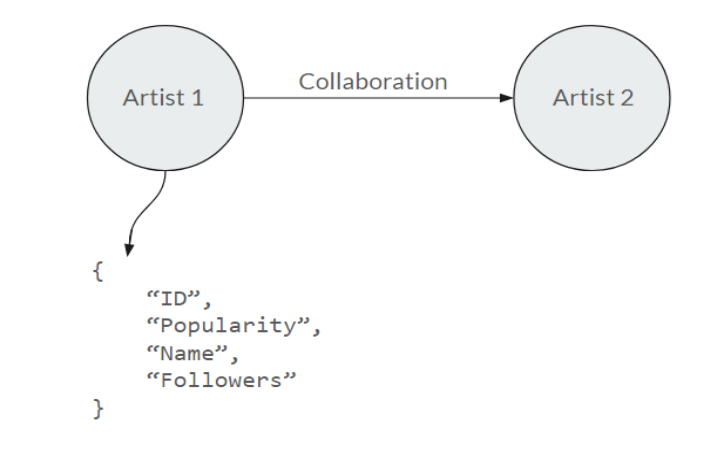
\includegraphics[width=0.6\textwidth]{node}
        \caption{Node \& Edge Visual}
        \label{fig:mesh1}
    \end{figure}\\
    All nodes within this network follow the setup of the diagram above with each artist node containing the following: id, popularity, name, and followers this is important for our undirected network because of the ability to have ids that link each node to another this is how our edges are created they are 1:1 edges from id to id if the individual has any song/album that they collaborated with another artist.
\section{Basic Statistics}
Below includes the following statistics for our network:
\begin{table}[H]
  \begin{center}
\begin{tabular}{ccc}
  \hline
  Measures &   \\
  \hline
  Number of nodes &  3040\\
  Number of edges & 3426\\
  Number of connected components & 3040\\
  Clustering coefficient & 0.204 \\
  Avgerage path length & 4.782 \\
  Graph Density & 0.001\\
  \hline
  \end{tabular}
\end{center}
  \caption{Basic statistics}\label{tab1}
  \end{table}
  \begin{figure}[H]
    \centering
    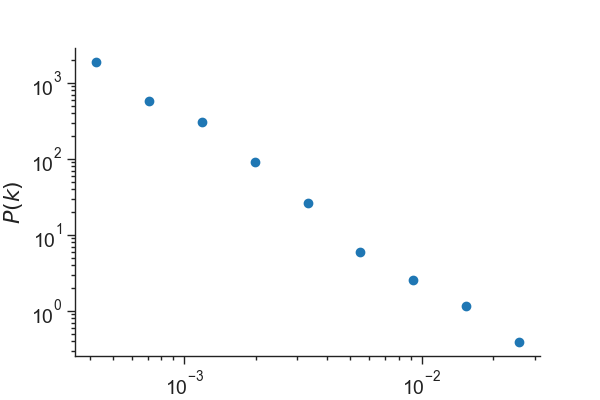
\includegraphics[width=0.75\textwidth]{degreedist}
    \caption{Degree Distribution}
\end{figure}
\section{Network Visualization}
\begin{figure}[H]
  \centering
  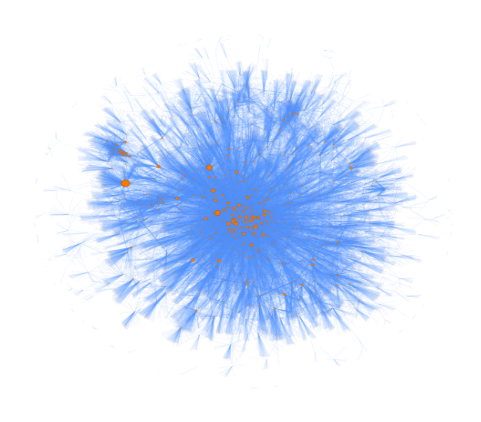
\includegraphics[width=0.75\textwidth]{entire2}
  \caption{Entire Network - 1}
\end{figure}

\begin{figure}[H]
  \centering
  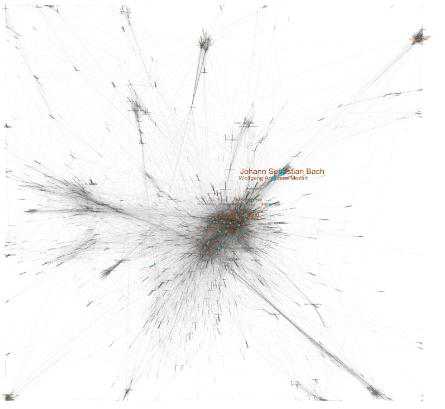
\includegraphics[width=0.7\textwidth]{entire1}
  \caption{Entire Network - 2}
\end{figure}

\begin{figure}[H]
  \centering
  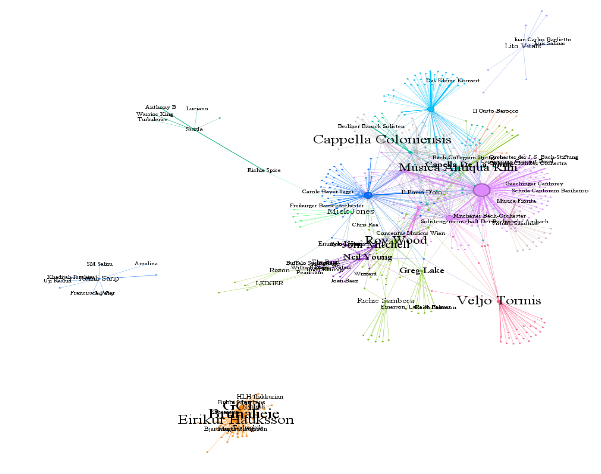
\includegraphics[width=0.75\textwidth]{english}
  \caption{Subset of 500 Artists}
\end{figure}

\begin{figure}[H]
  \centering
  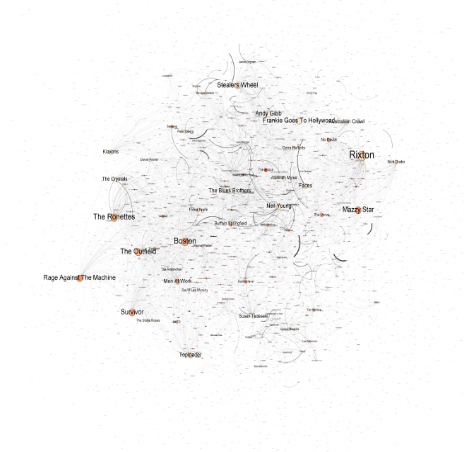
\includegraphics[width=0.75\textwidth]{subset2}
  \caption{Subset of English Artists - 1}
\end{figure}

\begin{figure}[H]
  \centering
  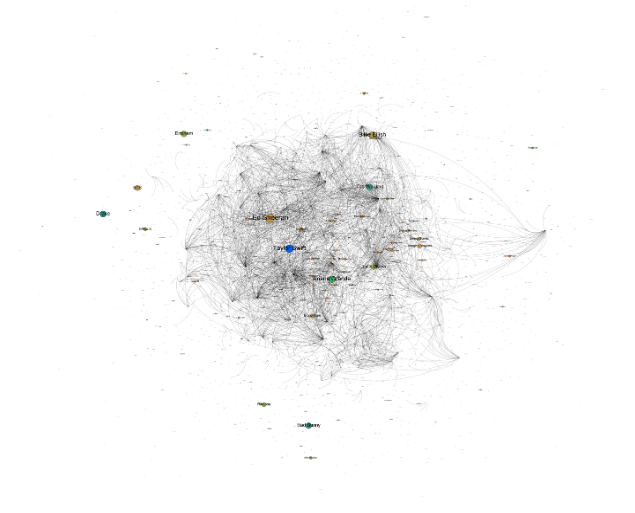
\includegraphics[width=0.75\textwidth]{subset}
  \caption{Subset of English Artists - 2}
\end{figure}
\section{Results}
\begin{enumerate}
  \item Who are the top artists when it comes to working together with others
\end{enumerate}
In Figure 6, the size of a node indicates the number of connections, and the node label's size is proportional to the node size. The larger the node, the clearer the label becomes. The node's color, changing from light orange to orange to red, illustrates the node's popularity change. The darker the color, the higher the popularity.\\

The predominance of orange hues and larger nodes suggests that individuals of medium popularity are more inclined to collaborate with each other. Thus, artists like Rage Against The Machine, Mazzy Star, and Boston are more likely to collaborate with other artists as they have the largest nodes in the graph. These artists tend to have a mid-level popularity, indicated by the node's color being somewhere between orange.\\

In Figure 7, the node size represents the number of fans, and the node label's size is proportional to the node size. The larger the node, the larger and clearer the label. The color gradient, from light purple through light blue, orange, green, to bright blue, signifies the change in the number of fans per node. As the color transitions, the larger the node, the greater the number of fans.\\

From this graph, it is evident that well-known artists like Taylor Swift and Ed Sheeran are less likely to collaborate with others. It logically follows that major artists might avoid collaborating with those who have fewer followers.\\

The Python script used to generate the top 10 in terms of degree centrality supports our assumption. With degree centrality and betweenness centrality values listed for artists like Mazzy Star, Rage Against The Machine, and Rixton, a higher degree centrality is indicative of more collaborations. Artists such as Rixton, Boston, and The Ronettes, with higher degrees of centrality, appear to be more connected than others on the list. Furthermore, a higher betweenness centrality suggests a stronger influence on the network's flow. For instance, Rixton, having a notably high betweenness centrality, likely plays a crucial role in connecting disparate groups or artists within the network.\\
\begin{enumerate}
  \setcounter{enumi}{1}
  \item Do artists who work with others a lot also get more famous?
\end{enumerate}
This question is challenging to address due to the limitations of our dataset in capturing changes in fame over time. To effectively analyze how artists "get more famous," we would require a more comprehensive dataset that tracks changes in popularity metrics. However, from the data we have, which includes metrics like the number of nodes (3040), number of edges (3426), average path length (4.782), average clustering coefficient (0.204), and graph density (0.001), we can draw some conclusions about the structure of the music industry network.\\

The average path length being less than 5 suggests a "small-world" effect within the network, meaning any two artists are, on average, separated by just a few steps despite the network's large size. This indicates a high degree of interconnectedness in the music industry, which could facilitate the rapid spread of trends, styles, or collaborative opportunities.\\

However, the graph density of 0.001 is very low, pointing to a sparse network. This sparsity could be due to the dataset's quality or reflect the reality that many potential connections between artists are not realized. In such a sparse network, achieving fame through a few collaborations might be challenging. It suggests that for artists to significantly increase their fame, collaborating with as many different artists as possible might be a more effective strategy. This approach could increase their visibility and connectivity within the network, potentially leading to more opportunities for exposure and recognition.
\begin{figure}[H]
  \centering
  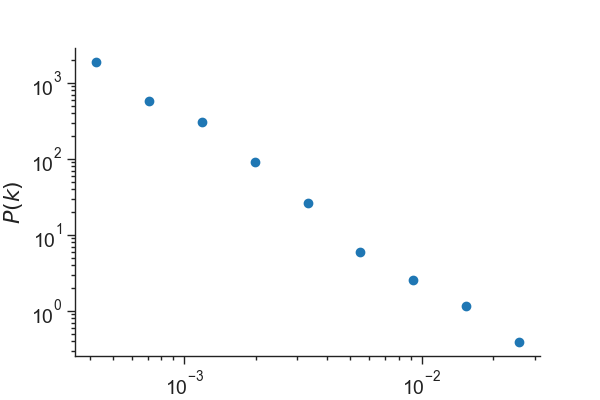
\includegraphics[width=0.75\textwidth]{degreedist}
  \caption{Degree Distribution of Figure 6 and 7}
\end{figure}
The overall downward trend suggests that nodes with a higher degree are less common, which is typical in most networks - as the degree increases, fewer nodes have that many connections. For artists, this could mean that the path to increasing their popularity and influence may involve not just producing quality music but also strategically increasing their visibility and connections within the network.
\section{Comparison to Suitable Null Model}
\begin{figure}[H]
  \centering
  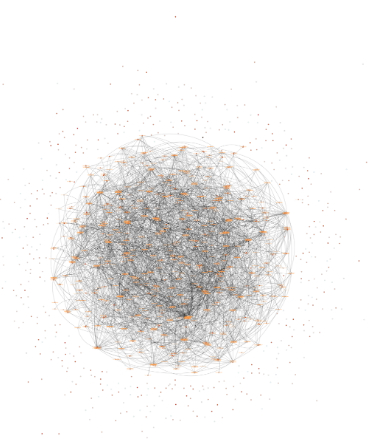
\includegraphics[width=0.75\textwidth]{null}
  \caption{Null Model}
\end{figure}
\textbf{Explanation of this Null Model}
\begin{enumerate}
  \item The size of the node indicates the number of connections, and the node label is proportional to the node size. The larger the node, the clearer the label;
  \item The color of the node, the gradient from light orange to orange to red, illustrates the change in the popularity of the node. The darker the color, the higher the popularity. There are more oranges in the figure and the nodes are larger, indicating that people with medium popularity are more likely to cooperate with each other.
  \item The node label color is the same as the node color and has no special meaning, which is convenient for displaying changes in popularity. The thickness of the edge indicates the frequency of cooperation;
\end{enumerate}
\begin{table}[H]
  \begin{center}
\begin{tabular}{ccc}
  \hline
  Measures &   \\
  \hline
  Number of nodes &  3040\\
  Number of edges & 4557 (+1517)\\ %3426
  Number of connected components & 3040\\
  Clustering coefficient & 0.001 (-0.203) \\ %0.204
  Avgerage path length & 6.11 (+1.328) \\ %4.782
  Graph Density & 0.001\\
  \hline
  \end{tabular}
\end{center}
  \caption{Null Model Statistics}\label{tab1}
  \end{table}
\begin{figure}[H]
  \centering
  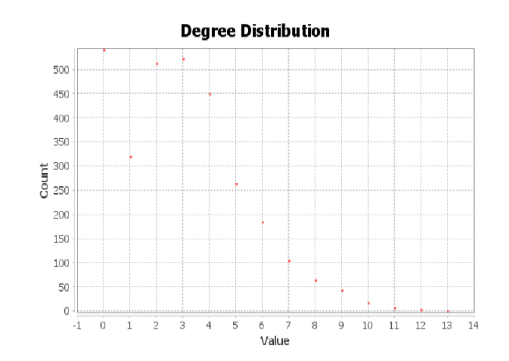
\includegraphics[width=0.75\textwidth]{degree}
  \caption{Degree Distibution Null Model}
\end{figure}
The regular model's higher average clustering coefficient (0.204 vs. 0.001 in the null model) and shorter average path length indicate a compact, "small-world" network. This suggests artists are more interconnected, forming tight-knit communities where collaboration or influence can spread quickly and easily, a characteristic common in social networks like those in the music industry.
\section{Discussion}
In our investigation into the collaborative networks of artists, we have adopted a refined dataset to gain insights into the intricate web of relationships that shape musical innovation and popularity. Comparing our findings with established literature, we see parallels with studies that identify collaboration as a key driver for artistic creativity and success (Cattani and Ferriani, 2008; Uzzi and Spiro, 2005). Our network's low-density points to a vast potential for new collaborative ventures, a characteristic underscored by Uzzi and Spiro in their exploration of Broadway creative networks.\\

Upon analysis, we have discovered that there are surprisingly short paths of collaboration on average, suggesting a 'small world' phenomenon within the artist network. However, the lower-than-expected clustering coefficient leads us to speculate that while some clusters of tight-knit collaboration exist, they are not widespread.\\

Our research questions aimed to uncover the most influential genres and artists in terms of collaborations and whether increased collaboration is linked to an increase in popularity. The lack of data on genre-specific collaborations presents a limitation, which means the question regarding genre influence remains partially unanswered. Despite this, our network metrics have allowed us to identify highly connected artists, which could serve as a proxy for influence, albeit incomplete without the genre context. Artists like Jonathan Sebastian Bach and Mozart have the highest degree centrality, which means they have the most collaborations and therefore the most influence in terms of collaborations. \\

For future work, constructing a multi-layered network incorporating genres as nodes connected by edges representing collaborations would enhance our understanding of genre-specific influences. Furthermore, integrating comprehensive popularity indices, such as streaming counts or social media metrics, would refine our analysis of the relationship between collaborations and artist popularity. Cross-referencing our findings with economic models could also shed light on the commercial implications of artist collaborations. As we strive for a holistic understanding, expanding our dataset to include global collaborations is an avenue for further exploration, potentially revealing the universality or specificity of our current findings.

\section{Methods}
To determine the most influential artists in terms of collaborations in our network, we focused on network centrality measures. These measures can help identify the most important or influential nodes (in our case, artists) within the network. With our network size, (48,651 nodes and 87,063 edges), here are the key centrality measures we calculated using NetworkX:\\

\textbf{Degree Centrality}: This is the simplest measure of node influence. It is based on the number of connections (collaborations) an artist has. In our collaboration network, a high degree of centrality means the artist has collaborated with many other artists.\\

\textbf{Betweenness Centrality}: This measure indicates how often a node appears on the shortest paths between other nodes. Artists with high betweenness centrality can be seen as influential in connecting different groups or clusters within the network.\\

\textbf{Closeness Centrality}: This reflects how close a node is to all other nodes in the network. It indicates how closely connected an artist is to the network as a whole, potentially influencing a broader range of artists.\\

\textbf{Eigenvector Centrality}: This measure considers not just the number of connections an artist has, but also the quality of these connections. It means that being connected to artists who themselves are highly connected is beneficial for an artist’s centrality score.\\

An artist scoring high across multiple centrality measures can be considered particularly influential.  For instance, an artist with high degree centrality but lower betweenness might be influential within a certain genre or community but not as much across different music communities. The code block below outlines the usage of Python library, Networkx, in calculating different centrality measures. Parallel processing was implemented to optimize the calculation of betweenness centrality.\\

\begin{lstlisting}[language=Python, caption=Python example]
  def calculate_betweenness_centrality(G, k=None):
    return nx.betweenness_centrality(G, k=k, normalized=True)

  def main():
    # Read data efficiently
    nodes = pd.read_csv('nodes_Copy.csv')
    edges = pd.read_csv('edges.csv')

    
    G = nx.from_pandas_edgelist(edges, 'Source', 'Target')

    #add node attributes
    nodes = nodes.drop_duplicates(subset='id')
    attr_dict = nodes.set_index('id').to_dict('index')
    nx.set_node_attributes(G, attr_dict)

    print(f"Number of nodes: {G.number_of_nodes()}")
    print(f"Number of edges: {G.number_of_edges()}")

    # Calculate degree centrality
    degree_centrality = nx.degree_centrality(G)

    # Parallel processing for betweenness centrality to reduce runtime
    pool = multiprocessing.Pool(processes=multiprocessing.cpu_count())
    betweenness_centrality = pool.apply(calculate_betweenness_centrality, args=(G, 1000))
    pool.close()
    pool.join()

    # other centralities
    closeness_centrality = nx.closeness_centrality(G)
    eigenvector_centrality = nx.eigenvector_centrality(G, max_iter=1000)

    # Sort and get top 10 for each centrality measure
    top_centralities = { 
        'degree': sorted(degree_centrality.items(), key=lambda x: x[1], reverse=True)[:10],
        'betweenness': sorted(betweenness_centrality.items(), key=lambda x: x[1], reverse=True)[:10],
        'closeness': sorted(closeness_centrality.items(), key=lambda x: x[1], reverse=True)[:10],
        'eigenvector': sorted(eigenvector_centrality.items(), key=lambda x: x[1], reverse=True)[:10]
    }


  \end{lstlisting}
\section{Code}
Our code in which we mainly used for creating our data and making our visualizations are available on our \href{https://github.com/Ty-Irving/CPSC-572-Project}{Github} the following 
table demonstrates what each file was used for. 
\begin{table}[H]
\centering
\resizebox{\textwidth}{!}{
\begin{tabular}{|l|l|}
\hline
File Name                      & File Description \\ \hline
NetworkAnalysis.py             &  Creates the degree distribution graph with the library networkx                \\ \cline{2-2} 
fetchalbums.py                 &  Fetches all of the artists albums and creates an edge list.                \\ \cline{2-2} 
fetchdata.py                   &  Creates a node list containing all the artists information.                \\ \cline{2-2} 
handle\_edges.py               &  Cleans edges file and creates a new edge list.                \\ \cline{2-2} 
handle\_nodes.py               &   Cleans node file and creates a new node list.               \\ \cline{2-2} 
networkStatTest.py             &   Calculates metrics about our network and creates files based on it.               \\ \hline
\end{tabular}
}
\caption{Code file descriptions}
\label{tab:my-table}
\end{table}

\begin{thebibliography}{9}
\bibitem{pee}
Peechapat, W., \& Puttanapong, N. (2024). Collaboration and Competition: A Social Network Analysis of Thailand’s Music Industry. \textit{Economies, 12}(2), 45. \url{https://doi.org/10.3390/economies12020045}
\bibitem{deshmane}
Deshmane, A., \& Martínez-de-Albéniz, V. (2023). Come Together, Right Now? An Empirical Study of Collaborations in the Music Industry. \textit{Management Science}. Advance online publication. \url{https://doi.org/10.1287/mnsc.2023.4743}
\bibitem{cattani}
Cattani, G., \& Ferriani, S. (2008). A Core/Periphery Perspective on Individual Creative Performance: Social Networks and Cinematic Achievements in the Hollywood Film Industry. \textit{Organization Science, 19}(6), 824-844.
\bibitem{uzzi}
Uzzi, B., \& Spiro, J. (2005). Collaboration and Creativity: The Small World Problem. \textit{American Journal of Sociology, 111}(2), 090090. Retrieved from VSJ.
\end{thebibliography}
\end{document}
